\documentclass[twocolumn]{article}

\usepackage{enumerate}
\usepackage{graphicx}
\usepackage[colorlinks=true,linkcolor=blue]{hyperref}
\usepackage[table,xcdraw]{xcolor}
\usepackage[english,spanish]{babel} 
\usepackage{helvet}
\usepackage{float}

\renewcommand{\familydefault}{\sfdefault}

\newenvironment{poliabstract}[1]
   {\renewcommand{\abstractname}{#1}\begin{abstract}}
   {\end{abstract}}

\begin{document}

\title{\Huge Comparativa de gestores de bases de datos no relacionales}
\author{
  Mejía Rodriguez, Julio Oliver\\
  \texttt{(2010037899)}
  \and
  Paredes Catacora, Randi Angel\\
  \texttt{(2013047246)}
  \and
  Herrera Amezquita, Derian Francisco\\
  \texttt{(2017059489)}
  \and
  Lipa Calabilla, Abraham\\
  \texttt{(2019064039)}
}
\date{30 de Noviembre de 2020}

\maketitle

\selectlanguage{spanish}
\begin{poliabstract}{Resumen} 
  En el mundo de las bases de datos, es importante conocer las diferentes alternativas que están disponibles para tomar la mejor decisión de acuerdo al problema que queremos dar solución. Uno de los puntos de discusión más importantes es el del rendimiento, facilidad de uso y la durabilidad del gestor de base de datos.

  En el presente trabajo se van a ver las características más importantes de los gestores de bases de datos no relacionales MongoDB y Redis, siendo estos los más populares. Veremos una comparación de sus características en común y los puntos en los que cada uno destaca más. Se van a comparar en rendimiento, facilidad de uso y la durabilidad del gestor de base de datos. Finalmente vamos a determinar los casos de uso de estos dos gestores de bases de datos.
\end{poliabstract}

\selectlanguage{english}
\begin{poliabstract}{Abstract} 
  In the world of databases, it is important to know the different alternatives that are available to make the best decision according to the problem we want to solve. One of the most important talking points is the performance, ease of use, and durability of the database manager.

  In this work, the most important characteristics of the non-relational database managers MongoDB and Redis will be seen, these being the most popular. We will see a comparison of their common characteristics and the points in which each one stands out the most. They will be compared in performance, ease of use and the durability of the database manager. Finally we are going to determine the use cases of these two database managers.
\end{poliabstract}

\section{Introducción}


\section{Bases de datos}

Una base de datos no es nada más que una colección de información que existe a lo largo de un periodo de tiempo, generalmente por muchos años.

El término ``database" se refiere a una colección de datos que son manejados por un \textit{Sistema gestor de base de datos} (o simplemente, Gestor de base de datos o \textbf{DBMS}). [1]

De un DBMS se espera:

\begin{itemize}
  \item Que los usuarios puedan crear nuevas bases de datos, consultar y modificar los datos ubicados en éstas, usando un lenguaje de definición, de consultas y de manipulación de datos, respectivamente.
  \item Que soporten el almacenamiento de grandes cantidades de información, así como la persistencia, el acceso eficiente y la recuperación.
  \item Que controle el acceso a los datos otorgado a los usuarios y que evite las acciones parciales sobre los datos.
\end{itemize}

Las bases de datos tradicionales están siendo utilizadas desde los 70's y su trabajo consiste en almacenar una gran cantidad de datos y obteniendo datos de múltiples tablas mediante uniones (\textit{`joins'}) complejas. [2]

Por 1990, las bases de datos relacionales fueron la norma. Las operaciones realizadas sobre los datos de una base de datos relacional se podían realizar mediante SQL (Lenguaje Estructurado de Consultas), el cual fue el más importante basado en el modelo relacional. [1]

\section{Bases de datos no relacionales}

\begin{description}
  \item[NoSQL] Se refiere a `No solo SQL' o simplemente `No SQL'. Describe tecnologías para el almacenamiento de datos que permiten la persistencia de datos con un alto rendimiento necesario para las aplicaciones de la escala de Internet de la actualidad. [3]
\end{description}

Una base de datos no relacional (o bases de datos NoSQL) responde a las necesidades de desarrollo de las aplicaciones modernas. [4]

\begin{itemize}
  \item Las aplicaciones generan enormes volúmenes de datos nuevos y en constante evolución (estructurados, semiestructurados, no estructurados y polimórficos).
  \item El trabajo se realiza en equipos pequeños, que realizan `sprints' de desarrollo ágiles con iteraciones rápidas.
  \item Las aplicaciones sirven como servicios, que no solo deben funcionar sin interrupción, sino que además tienen que ser accesibles desde muchos dispositivos distintos y deben poder escalarse.
  \item Las organizaciones ahora están recurriendo a arquitecturas de escalamiento horizontal que utilizan tecnologías de software abierto, servidores básicos y computación en la nube.
\end{itemize}

\subsection{Tipos de bases de datos NoSQL}

\begin{enumerate}

  \item Clave/Valor \\
        Los datos usan claves que son identificadores y que son similares a una llave primaria en una base de datos relacional. [3] Cada elemento de la base de datos se almacena como un nombre de atributo (o clave), junto con su valor. [4] Algunos ejemplos de este tipo son \textbf{Riak } y \textbf{Berkeley DB}.

  \item Orientadas a columnas \\
        Los datos se organizan por columnas en lugar de por filas. El efecto de este diseño arquitectónico es que hace que las consultas agregadas sobre grandes cantidades de datos sean mucho más rápidas de procesar. [3] Algunos ejemplos de este tipo son \textbf{Cassandra} y \textbf{HBase}.

  \item Documentos \\
        Se empareja cada clave con una estructura de datos compleja que se denomina `documento'. Los documentos pueden contener muchos pares de clave-valor distintos, o pares de clave-matriz, o incluso documentos anidados. [4] Un ejemplo de este tipo es \textbf{MongoDB}.

  \item Grafos \\
        Utilizan la teoría de grafos para almacenar relaciones de datos en una serie de vértices con aristas, lo que hace que las consultas que funcionen con datos de esta manera sean mucho más rápidas. [3] Algunos ejemplos de este tipo son \textbf{Neo4J} y \textbf{Giraph}.

\end{enumerate}

\section{MongoDB}

MongoDB es una base de datos NoSQL basado en documentos JSON y de código abierto escrito en C++, que proporciona alto rendimiento, alta disponibilidad y escalabilidad automática. [5]

Las bases de datos como MongoDB proporcionan escalabilidad automática, lo cual hace que esta base de datos sea idónea para grandes cantidades crecientes de información. [5]

El desarrollo de MongoDB comenzó en el año 2007 por la empresa 10gen3, publicando una versión final en el 2009 y actualmente se encuentra en la versión 4.4. [5]

\subsection{RDBMS y MongoDB}

A continuación se muestra una comparación de los términos utilizados en ambos tipos de bases de datos solo a modo orientativo, dado que no cuentan con la misma estructura. [6]

\begin{table}[h]
\centering
\begin{tabular}{|l|l|}
\hline
\rowcolor[HTML]{67FD9A} 
\textbf{RDBMS} & \textbf{MongoDB}               \\ \hline
Database       & Database                       \\ \hline
Table          & Collection                     \\ \hline
Tuple/Row      & Document                       \\ \hline
Column         & Field                          \\ \hline
Table Join     & Embedded Documents             \\ \hline
Primary Key    & Primary Key (Default key \_id) \\ \hline
\end{tabular}
\caption{Tabla comparativa de terminología RDMS - MongoDB}
\end{table}

\subsection{Ventajas sobre RDBMS}

Algunas de las ventajas que tiene MongoDB sobre los gestores de bases de datos relacionales son: [6]

\begin{itemize}
  \item Menos esquema
  \item La estructura de un objeto es clara
  \item No requiere de uniones complejas
  \item Consultas dinámicas sobre documentos
  \item Fácil escalabilidad
  \item No requiere de conversión o mapeo de objetos
  \item Rápido acceso a los datos
\end{itemize}

\subsection{Arquitectura}

En una base de datos de MongoDB, hay tres partes principales: [8]

\begin{description}
  \item[mongod (MongoDB server)] Es el proceso principal que maneja las solicitudes de datos, administra el formato de los datos y realiza operaciones de administración en segundo plano. Puede haber muchos demonios mongod ejecutándose como instancias primarias secundarias.
  \item[mongos] Es el servicio de enrutamiento. Este proceso enruta información y datos en el clúster.
  \item[MongoDB shell] Es la interfaz interactiva. Al usar JavaScript para ordenar, el desarrollador puede examinar los resultados de las consultas y verificar los casos de prueba.
\end{description}

\begin{figure}[h]
  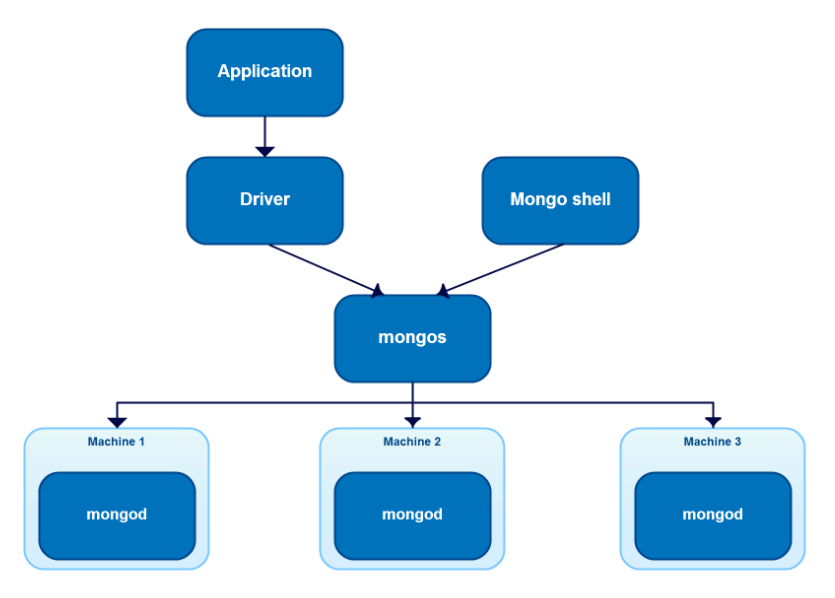
\includegraphics[width = \columnwidth]{img/01_mongo.png}
  \caption{Arquitectura de una base de datos MongoDB}
\end{figure}

\subsection{BSON}

Generalmente, los usuarios trabajan con MongoDB mediante el formato JSON, sin embargo, MongoDB usa BSON (o `Binary JSON'). BSON extiende del modelo JSON para proporcionar ``tipos de datos" para una correcta codificación y decodificación en los diferentes lenguajes. [5]

\subsubsection{JSON y BSON}

JSON proporciona únicamente 6 tipos de datos: [5]

\begin{itemize}
  \item String
  \item Number
  \item Booleans
  \item null
  \item Arrays
  \item Objetos / documentos
\end{itemize}

Los tipos de datos que maneja internamente BSON son los siguientes:

\begin{itemize}
  \item Double
  \item String
  \item Object
  \item Array
  \item Binary data
  \item Undefined (deprecated)
  \item Object id
  \item Boolean
  \item Date
  \item Null
  \item Regular Expression
  \item JavaScript Symbol JavaScript (con scope)
  \item 32-bit integer
  \item Timestamp
  \item 64-bit integer
  \item Min key
  \item Max key
\end{itemize}

\section{Redis}

Redis es una base de datos NoSQL, pero también, es una base de datos multi-modelo que permite la búsqueda, la mensajería, streaming, grafos y otras capacidades más allá de la de un simple almacén de datos. [3]

Redis mantiene los datos en la memoria para un acceso rápido y conserva los datos en el almacenamiento, así como la replicación de los contenidos en la memoria para escenarios de producción de alta disponibilidad. [3]

\subsection{Estructura}

\subsubsection{Bases de datos}

En Redis, al igual que en otras DBMS, una base de datos es un conjunto de datos. El caso de uso típico para una base de datos es agrupar los datos de una aplicación y mantenerlos separados de otras aplicaciones. [7]

\subsubsection{Clave / Valor}

Cada una de las estructuras de datos en Redis tienen al menos una clave y un valor. [7]

\begin{description}
  \item[Claves] Son cómo identificamos piezas de datos.
  \item[Valor] Representan los datos actualmente asociados con la clave.
\end{description}

\subsection{Almacenamiento de estructuras de datos}

Las estructuras de datos soportadas que se incluyen: [3]

\begin{itemize}
  \item Strings
  \item Lists
  \item Sets
  \item Sorted sets
  \item Hashes
  \item Bit arrays
  \item Streams
  \item HyperLogLogs
\end{itemize}

\subsection{Arquitectura}

La arquitectura de Redis está basada en el enfoque BASE (Disponible básicamente, Soft-state y eventualmente consistente) mientras se elimina el enfoque ACID (atomicidad, consistencia, durabilidad y aislamiento) en RDBMS. Redis se basa en la arquitectura cliente / servidor y consta de los siguientes componentes: [8]

\begin{itemize}
  \item Servidor Redis
  \item Servidores réplica de Redis (opcionales)
  \item Cliente Redis
\end{itemize}

\begin{figure}[h]
  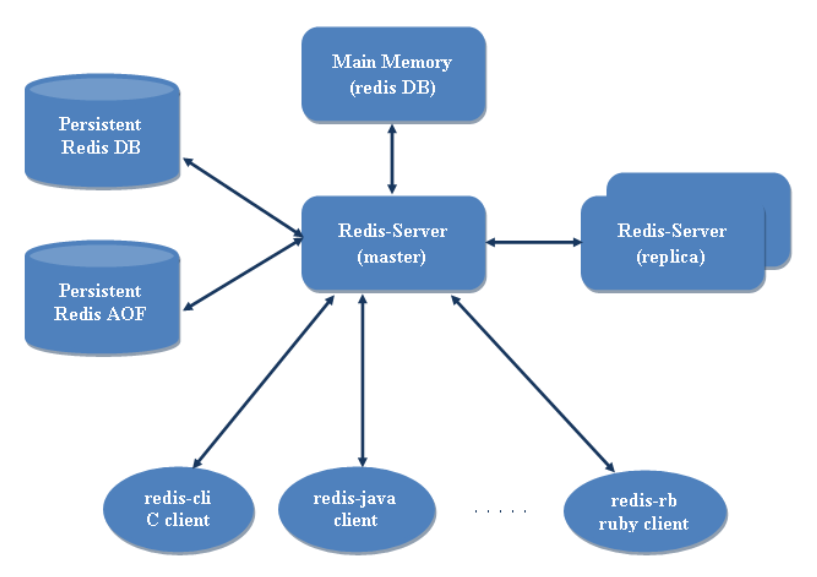
\includegraphics[width = \columnwidth]{img/02_redis.png}
  \caption{Arquitectura de una base de datos Redis}
\end{figure}

\section{Comparación}

Para la comparación de rendimiento entre MongoDB y Redis, se ha realizado un proceso de benchmarking en una sola máquina (con las mismas características). La herramienta utilizada es YCSB (Yahoo Cloud Serving Benchmark).

Versiones de las bases de datos:

\begin{description}
  \item[MongoDB] 2.7.4
  \item[Redis] 2.8.15
\end{description}

\subsection{Rendimiento}

Se muestran los datos correspondientes a la relación entre el número de hilos de la máquina (los cuales son 1, 2, 4 y 8) y las operaciones por segundo, dada cierta cantidad de registros (1000, 5000 y 10000) y 1000 operaciones realizadas.

\begin{figure}[H]
  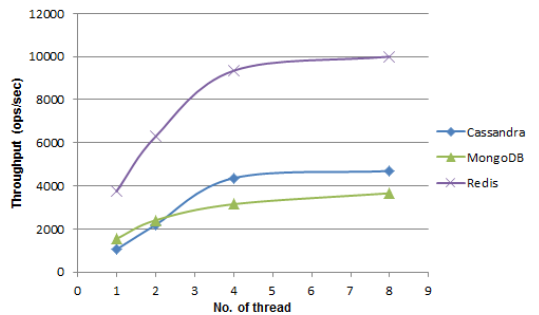
\includegraphics[width = \columnwidth]{img/03_g1.png}
  \caption{Gráfico comparativo con 1000 registros y 1000 operaciones}
\end{figure}

\begin{figure}[H]
  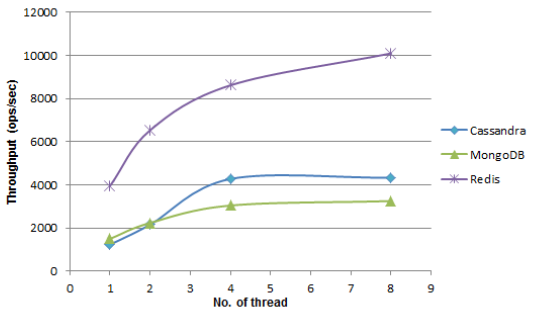
\includegraphics[width = \columnwidth]{img/04_g2.png}
  \caption{Gráfico comparativo con 5000 registros y 1000 operaciones}
\end{figure}

\begin{figure}[H]
  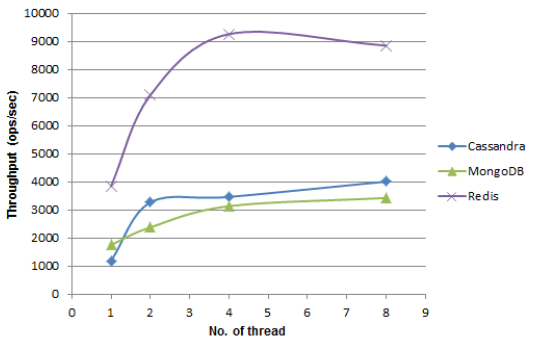
\includegraphics[width = \columnwidth]{img/05_g3.png}
  \caption{Gráfico comparativo con 10000 registros y 1000 operaciones}
\end{figure}

\subsection{Latencia y rendimiento}

Se muestran los datos correspondientes a la relación entre el número de hilos de la máquina (los cuales van desde 1 a 50) y la latencia en microsegundos, dados 100000 registros.

\begin{figure}[H]
  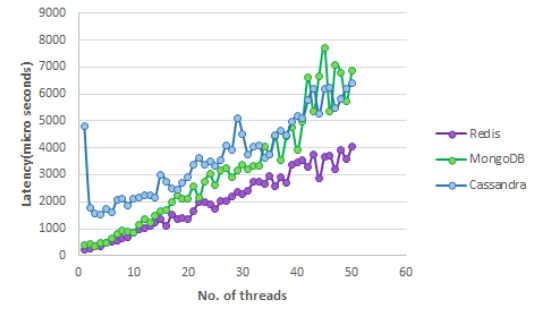
\includegraphics[width = \columnwidth]{img/06_g4.png}
  \caption{Latencia de lectura}
\end{figure}

\begin{figure}[H]
  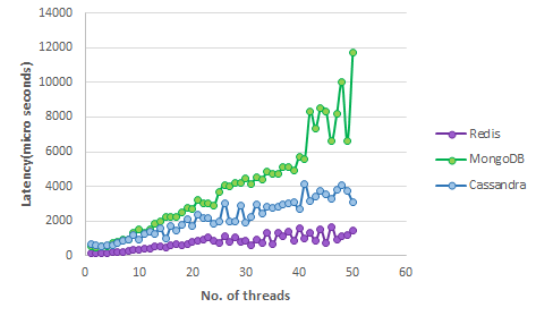
\includegraphics[width = \columnwidth]{img/07_g5.png}
  \caption{Latencia de actualización}
\end{figure}

Se muestran los datos correspondientes a la relación entre el número de hilos de la máquina (los cuales van desde 1 a 50) y las operaciones por segundo, dados 100000 registros.

\begin{figure}[H]
  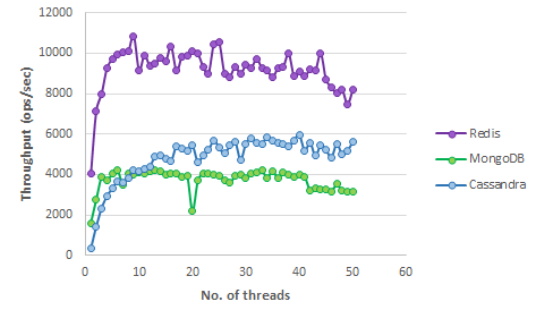
\includegraphics[width = \columnwidth]{img/08_g6.png}
  \caption{Rendimiento con 100000 registros}
\end{figure}

\section{Conclusiones}



\section{Recomendaciones}



\section{Bibliografía}



\end{document}